Finally, an addition step was included to the fiber conditioning process, with the objective of improving the photon collection efficiency of the fibers. 

The tritium events detected in the fibers produce few photons, so it is very important to conserve as many photons as possible. As it was shown in the fiber characterization study, the quality of the interface that is created between the core of no clad fibers and the environment (tritiated water in the case of TRITIUM detector) greatly affects the photon collection efficiency.

Therefore, a mechanism, called the fiber cleaning process, was applied to improve the state of this interface. This mechanism aims to remove all external particles deposited on the fibers, such as fat molecules deposited when the fibers are touched, which can affect the quality of the interface, worsening their photon collection efficiency. 

As a consequence of this cleaning process, the wetting property of the fibers, shown in Figure \ref{fig:WettingProperty}, is improved, preventing air molecules from attaching to the fiber and achieving a uniform water clad around each fiber, resulting in an improvement of their collection efficiency. 

%Therefore, a mechanism, called the fiber cleaning process, was applied. As we can see in Figure \ref{fig:WettingProperty}, this cleaning process was carried out to improve the wetting properties, preventing air molecules from attaching to the fiber and achieving a uniform water clad around each fiber, avoiding variations in its refractive index which can worsen the photon collection efficiency of the fibers.

\begin{figure}[h]
\centering
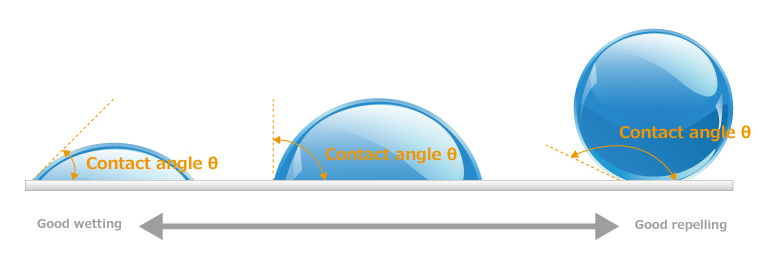
\includegraphics[scale=0.5]{4ResearchAndDevelopments/41Fibers/WettingProperty.png}
\caption{Wetting property produced by the cleaning process. \cite{WettingProperty}\label{fig:WettingProperty}}
\end{figure}


This cleaning process  was carried out within a clean room at ICMOL laboratories\footnote{ICMOL, Institute of Molecular Science, is a research institute located in the Science Park of the University of Valencia.} and it was developed by their researchers.

It consists of filling three different beakers, one with alkaline soap, another with millipore water\footnote{The millipore water is water in which all the ions were removed, producing a very low conductivity of it-self, on the order of $10~\mu\sievert/\cm^2$} and the last one with isopropanol. First, the fibers are rubbed for 5 minutes with alkaline soap and then placed in the first beaker for sonication for 3 minutes. Then, the fibers are cleaned with a constant flow of water for 5 minutes. Second, the fibers are placed in the second beaker for sonication for another 3 minutes. Third, the fibers are placed in the third beaker for sonication for another 3 minutes. Finally the fibers are dried with an $N_2$ air gun and introduced inside of the prototype.

The improvement in fiber response was verified using a bundle of twenty fibers with a length of $15~\cm$ that was prepared with the conditioning process previously described. This bundle of fibers was arranged in the setup described in section \ref{subsec:PolishingMachine}, Figure \ref{fig:BunchWith2PMTsCoincidence} and several measurements were taken. Then, these fibers were cleaned with the fiber cleaning process and these measurement was repeated in the same conditions.

Two radioactive sources were used in this study, a beta source, $\ce{^{90}Sr}$, which is the same as that used in the polishing machine test, and a gamma source, $\ce{^{137}Cs}$, the activity of which is of the order of $500~\becquerel$.

The results are shown in Figures \ref{fig:ResultsOfCleaningProcess}, where a shift of the spectrum to the right can be seen. 

\begin{figure}
\centering
    \begin{subfigure}[b]{0.76\textwidth}
    \centering
    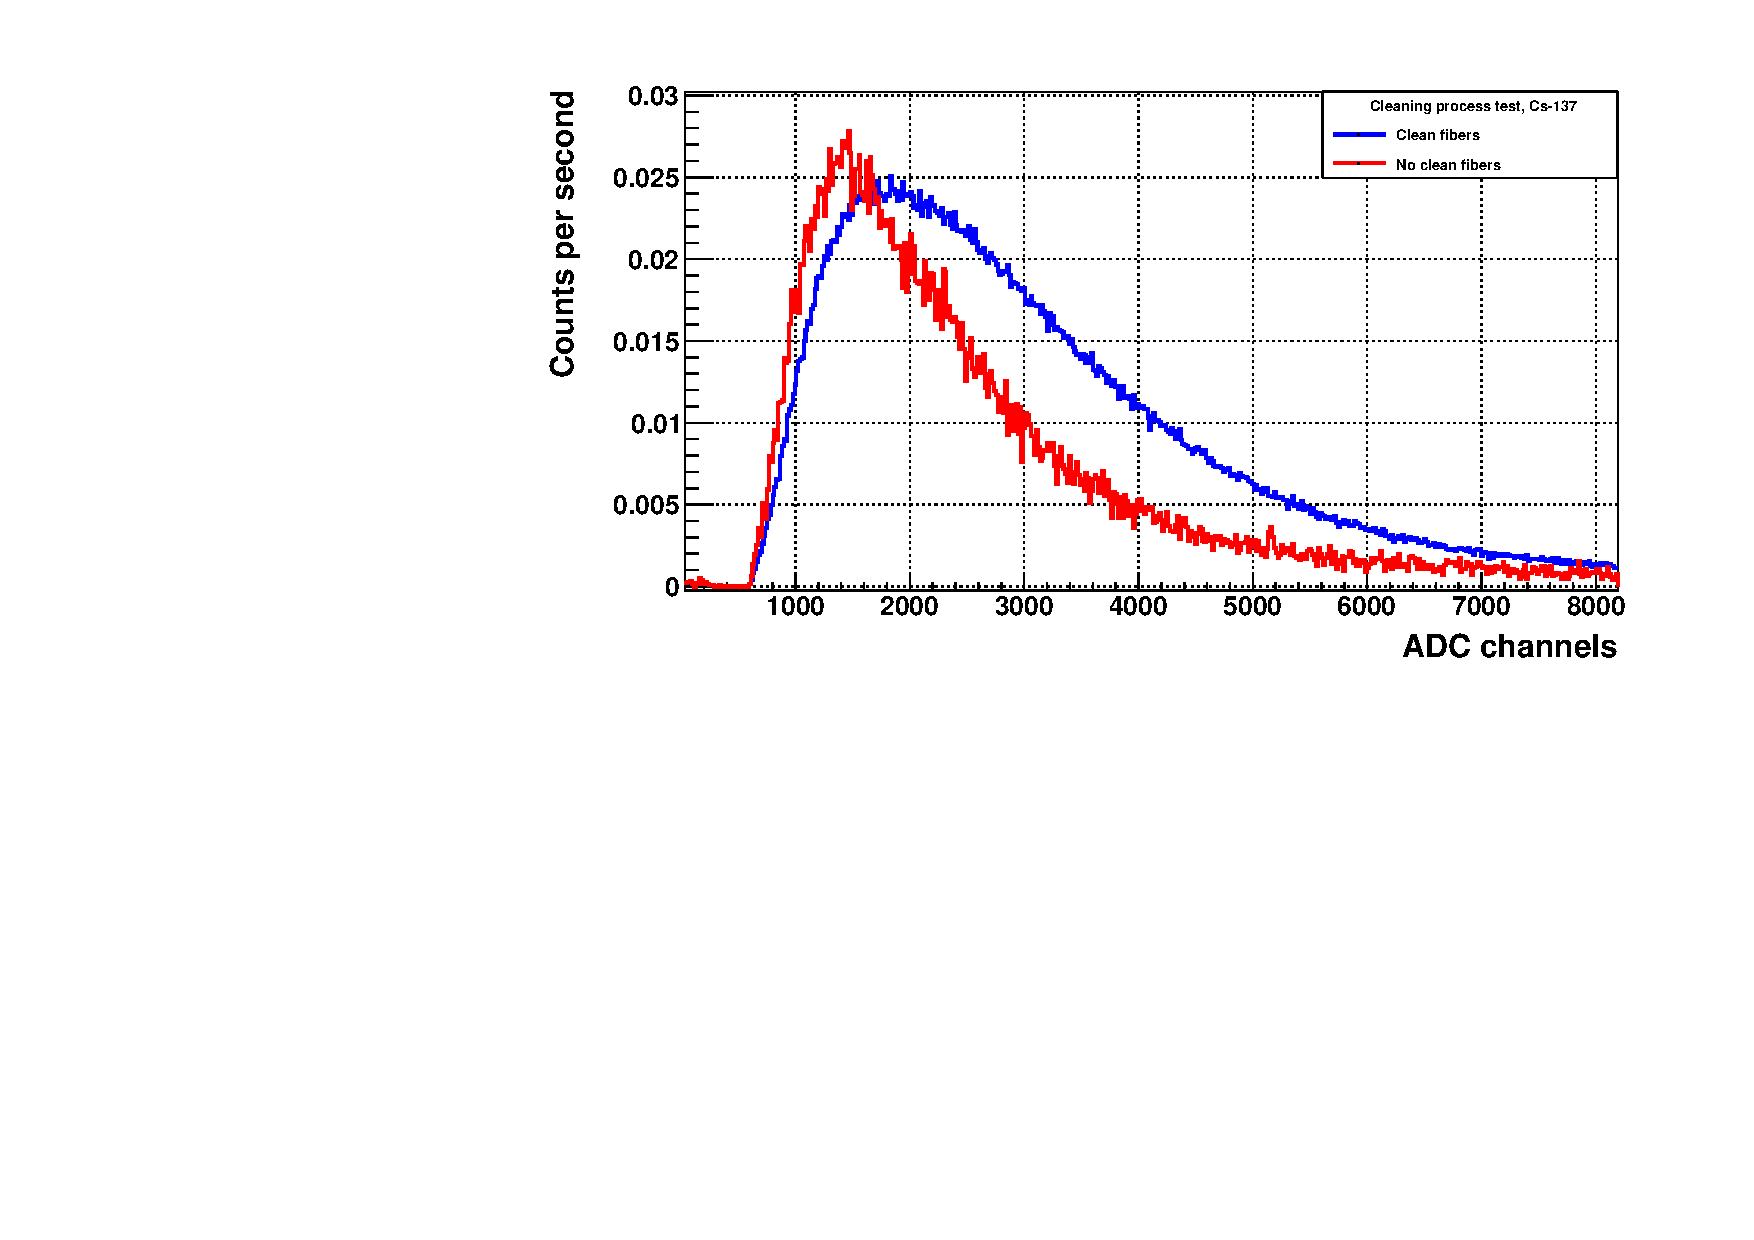
\includegraphics[width=\textwidth]{4ResearchAndDevelopments/41Fibers/Cs-137_CleaningProcess.pdf}  
    \caption{Energy spectrum recorded for the Cs-137 source.\label{subfig:EnergySpectrumCo60CleaningTest}}
    \end{subfigure}
    \hfill
    \begin{subfigure}[b]{0.76\textwidth}
    \centering
    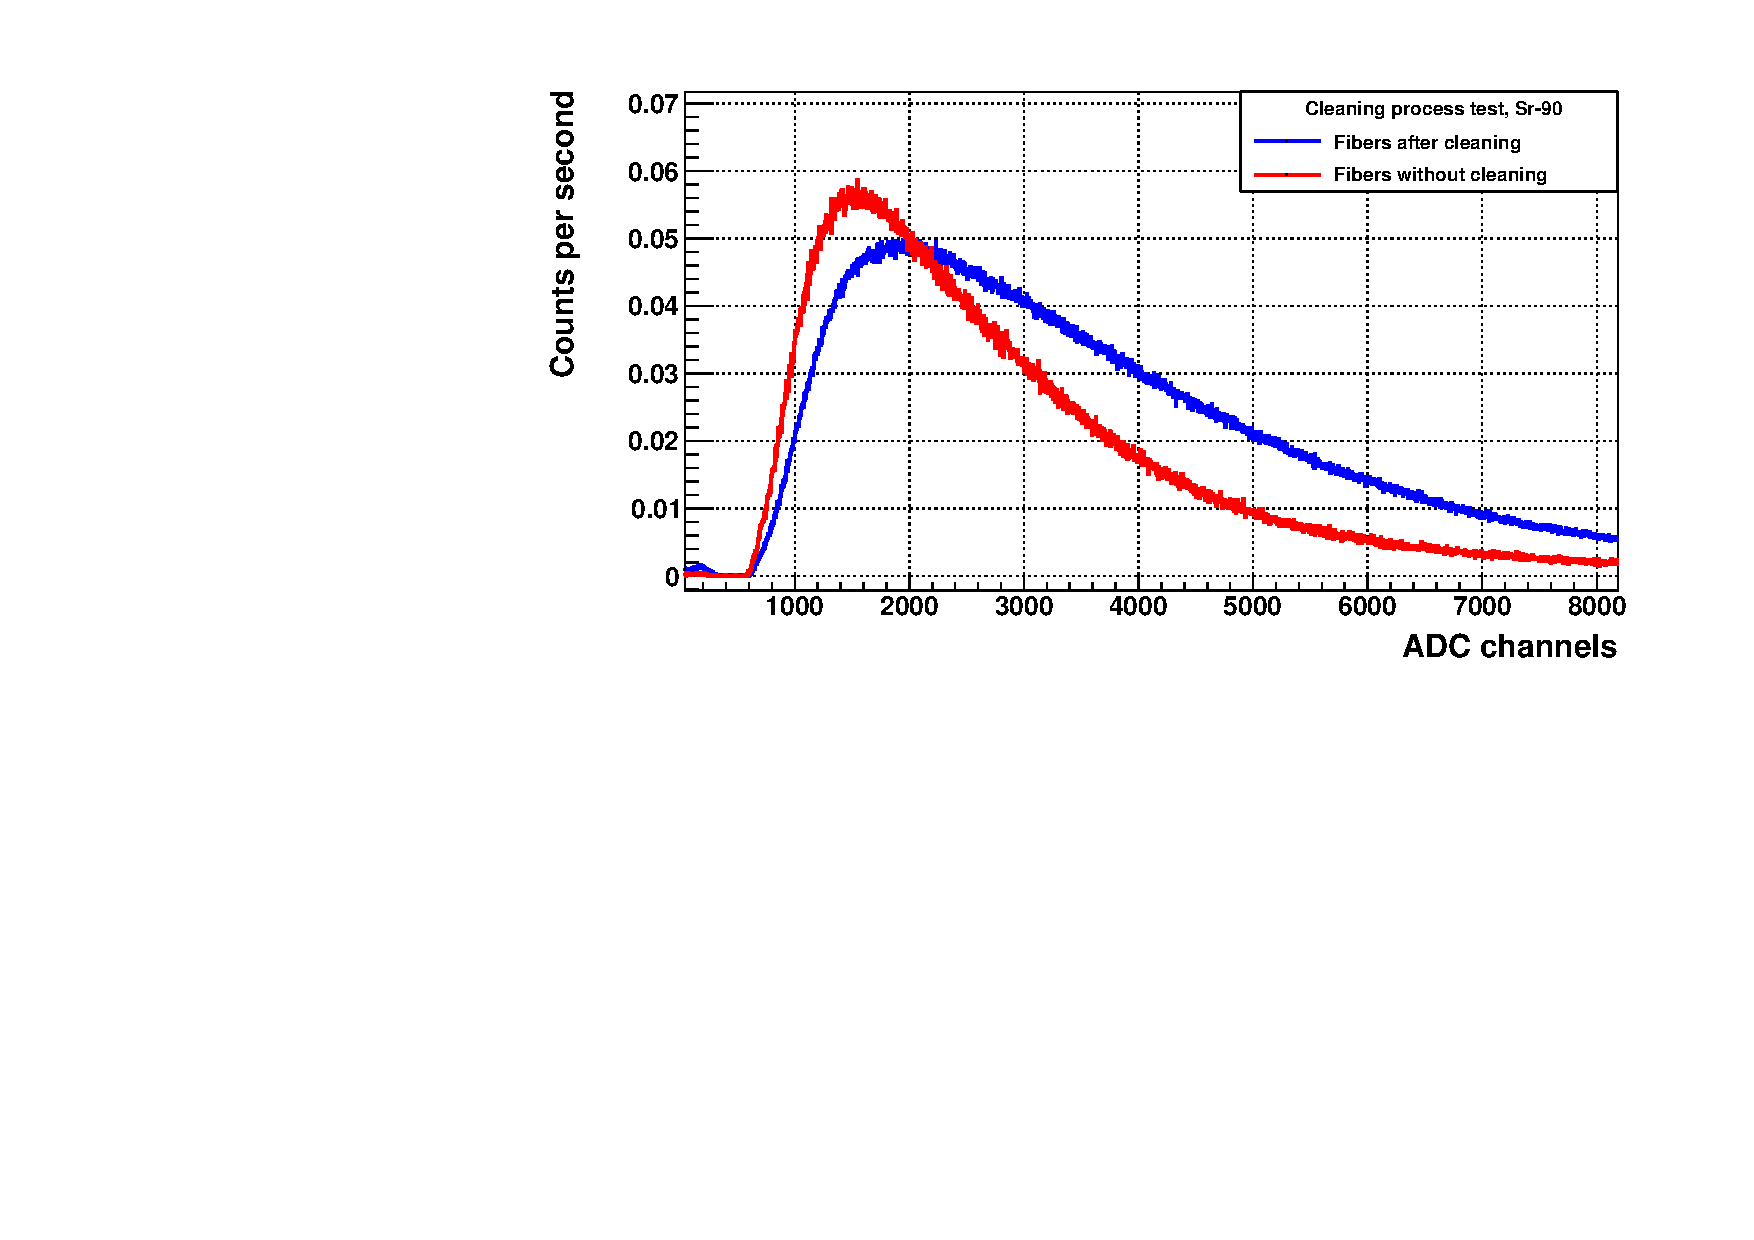
\includegraphics[width=\textwidth]{4ResearchAndDevelopments/41Fibers/Sr-90_CleaningProcess.pdf}  
    \caption{Energy spectrum recorded for the Sr-90 source.\label{subfig:EnergySpectrumSr90CleaningTest}}
    \end{subfigure}
 \caption{Energy spectrums used to test the effect of the Cleaning process}
 \label{fig:ResultsOfCleaningProcess}
\end{figure}

A rude approximation was done to quantify this improvement. It was calculated using the equation \ref{eq:RelativeImprovement}, where $A_{C}$ is the counts per second measured after the cleaning process and $A_{NC}$ is the counts per second measured before the cleaning process.

\begin{equation}
F(a,b)=\frac{A_{C}-A_{NC}}{A_{C}}
\label{eq:RelativeImprovement}
\end{equation}

The obtained improvement is $(27.73 \pm 1.6)\%$ for the gamma source and $(20.72 \pm 0.9)\%$ for the beta source so, the improvement of the photon collection efficiency of the fibers was verified using the cleaning process carried out in the clean room of ICMOL laboratories. Nevertheless, it should be taken into accout that this test was carried out in air. It could be interesting to repeat it in water to obtain more realistic conclusions since the fibers of the TRITIUM detector will be immersed in water.